%%%% Modelo de comportamiento %%%%

\section{Módulos}

	La figura \ref{modulos} muestra los módulos del sistema a desarrollar.


	A continuación se describe de manera general cada uno de los módulos.

	\begin{itemize}

		\item \textit{Selección de pizzas}. Permite al cliente visualizar funcionalidades como ver el catálogo de pizzas, seleccionarlas, ver su descripción y personalizarlas.

		\item \textit{Pago}. Permite al cliente visualizar funcionalidades como seleccionar su tipo de envío,  agregar información para su compra, seleccionar su método de pago y generar su PDF (comprobante de compra).
		

	\end{itemize}

	%Módulos del sistema
\begin{figure}[h]
	
	\begin{center}
		
		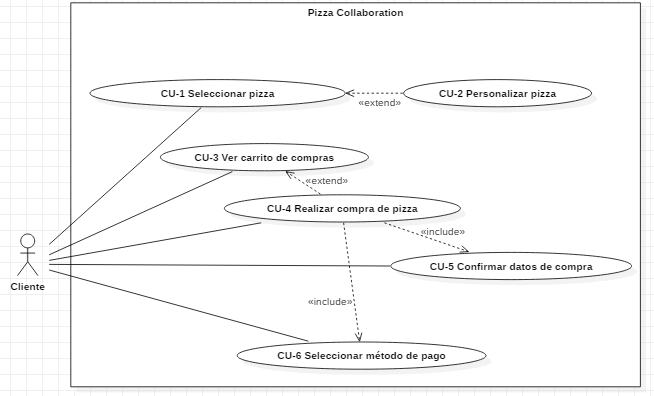
\includegraphics[scale=0.45]{imagenes/modulos/Modulos-PizzaCollaboration.png}
		\caption{Módulos del sistema}
		\label{modulos}
		
	\end{center}
	
\end{figure}

%\pagebreak[2]